\begin{itemize}
    \item Triangle centers
    \item Are Loci Algebraic (method of resultants)
    \item Are Loci Elliptic (Blaschke's parametrization \cite{daepp-2019})
    \item Monotonicity and Turning Number
    \item Table of results
\end{itemize}

Referring to Figure~\ref{fig:nonconcentric-xns}:

\begin{figure}
     \centering
     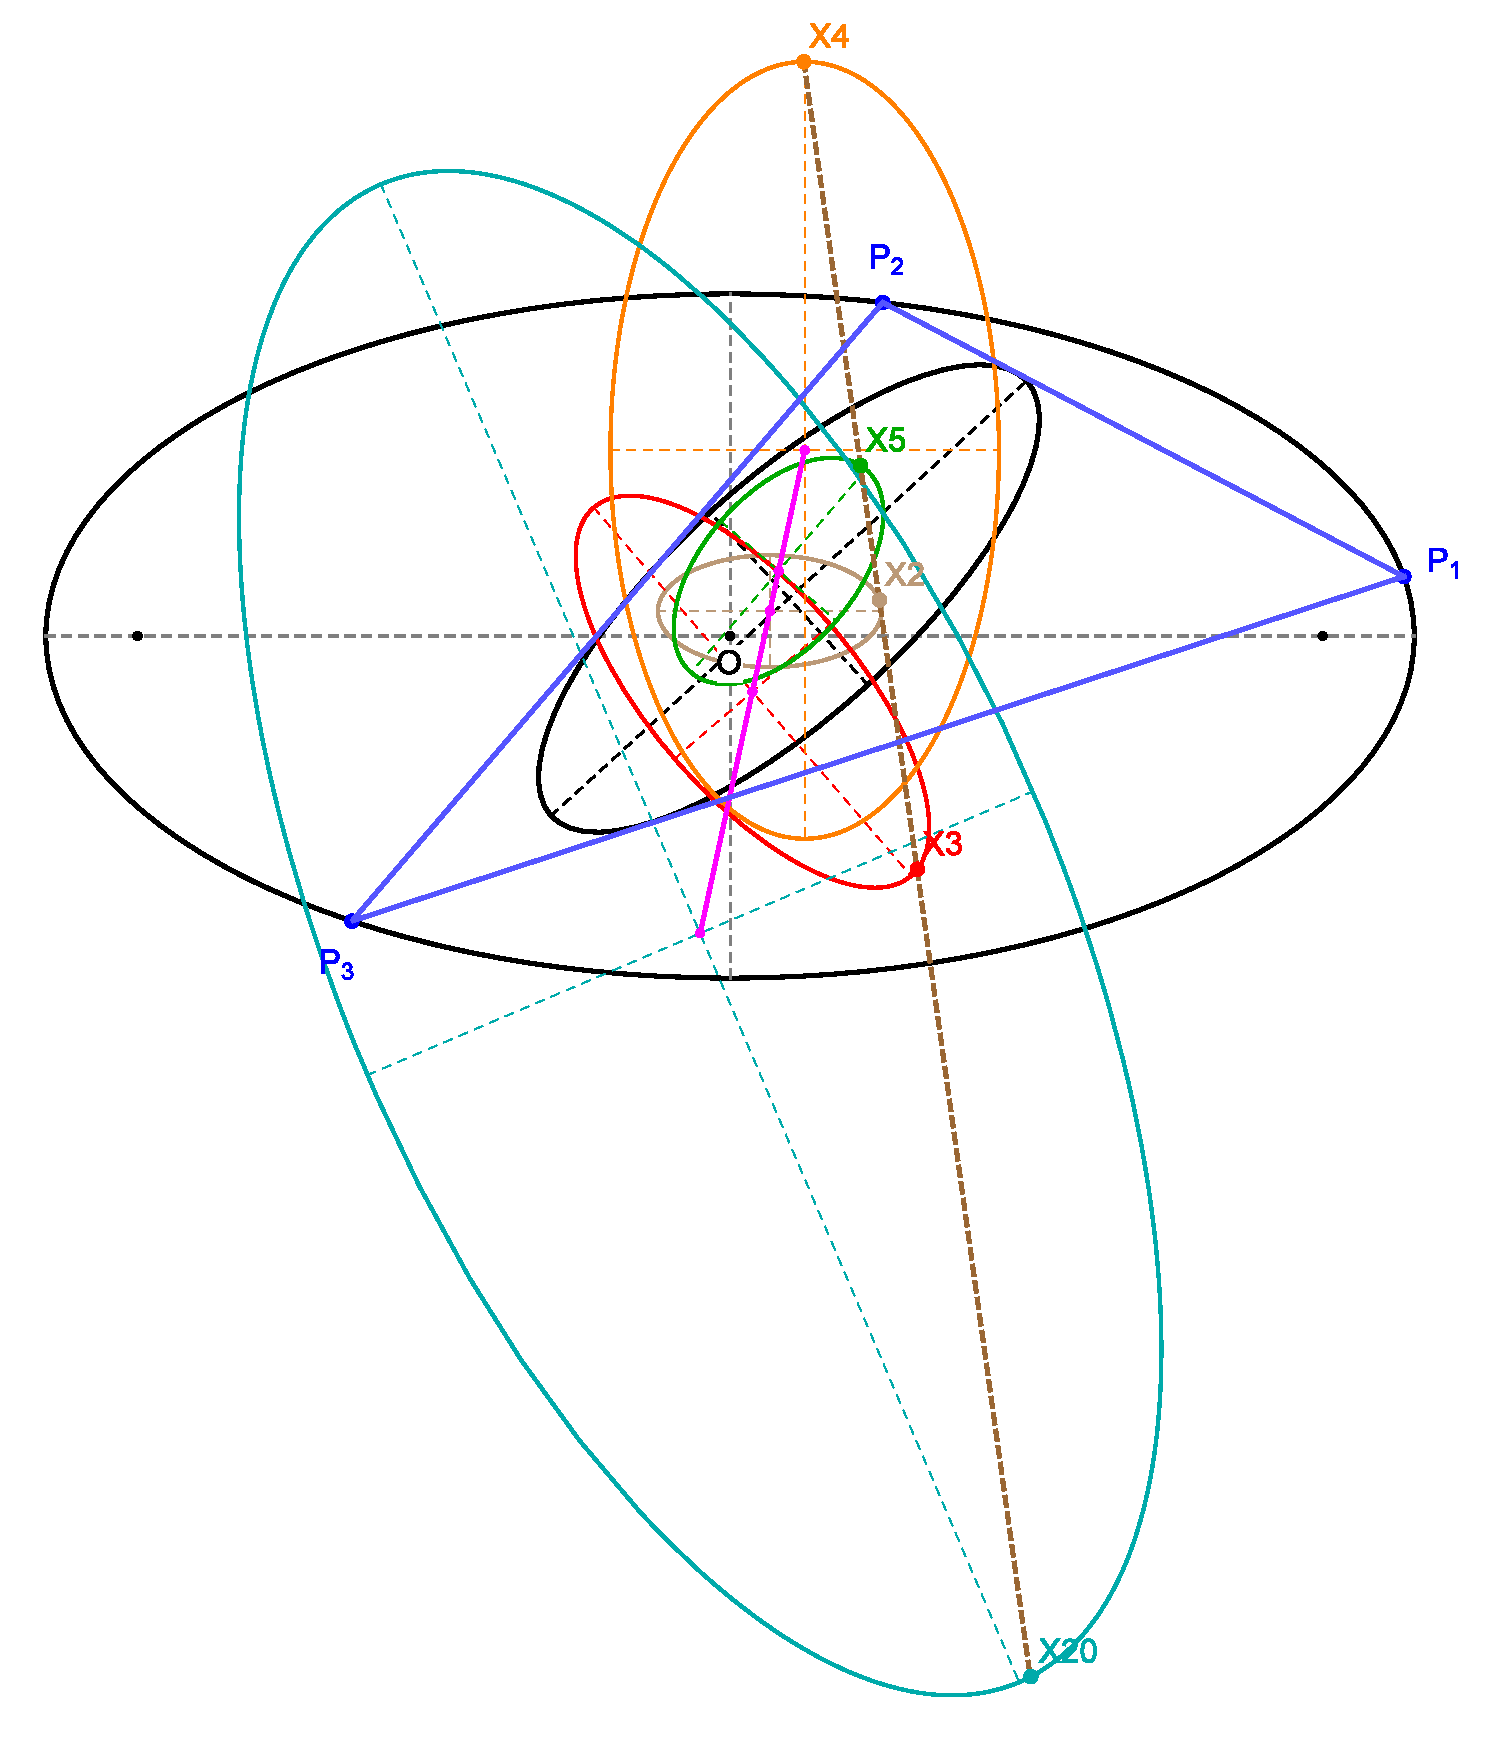
\includegraphics[width=.8\textwidth]{pics_03_010_n3_nonconcentric_conics.eps}
     \caption{A 3-periodic is shown interscribed between two non-concentric, non-aligned ellipses (black). The loci of $X_k$, $k=2,3,4,5,20$ (and many others) are elliptic. Those of $X_2$ and $X_4$ are axis-aligned with the outer ellipse. Furthermore, the centers of all elliptic loci are collinear (magenta line).}
     \label{fig:nonconcentric-xns}
 \end{figure}